\documentclass[aspectratio=169,10pt]{beamer}
\usetheme[progressbar=frametitle,numbering=fraction]{metropolis}
\usepackage[T1]{fontenc}
\usepackage{lmodern}
\usepackage{amsmath,amssymb,bm,booktabs,graphicx,xcolor,tikz,multicol}
\usetikzlibrary{arrows.meta,positioning,shapes.geometric,fit,backgrounds,calc}
\graphicspath{{../../validation/figures/}}

% ------------------------------------------------------------------ palette
\definecolor{oDark}{HTML}{14213D}
\definecolor{oAccent}{HTML}{8E3B8A}
\setbeamercolor{frametitle}{bg=oDark,fg=white}
\setbeamercolor{progress bar}{fg=oAccent,bg=oAccent!20}
\setbeamercolor{alerted text}{fg=oAccent}
\setbeamercolor{title separator}{fg=oAccent}

% ------------------------------------------------------------------ colour code for physical quantities
\definecolor{cE}{HTML}{1F5FA8}   % energies
\definecolor{cMu}{HTML}{C0392B}  % mobility / diffusion
\definecolor{cF}{HTML}{1E8449}   % field / potential
\definecolor{cT}{HTML}{D68910}   % temperature / thermal energy
\definecolor{cN}{HTML}{7D3C98}   % densities / occupations
\definecolor{cW}{HTML}{117A65}   % rates
\definecolor{cJ}{HTML}{2874A6}   % currents
\definecolor{cG}{HTML}{A04000}   % generation / recombination
\definecolor{cOp}{HTML}{6E2C00}  % operators
\definecolor{cX}{HTML}{5D6D7E}   % geometry (r, x, a)
\newcommand{\En}[1]{{\color{cE}#1}}
\newcommand{\Mu}[1]{{\color{cMu}#1}}
\newcommand{\Fd}[1]{{\color{cF}#1}}
\newcommand{\Tk}[1]{{\color{cT}#1}}
\newcommand{\Dn}[1]{{\color{cN}#1}}
\newcommand{\Rt}[1]{{\color{cW}#1}}
\newcommand{\Js}[1]{{\color{cJ}#1}}
\newcommand{\GR}[1]{{\color{cG}#1}}
\newcommand{\Op}[1]{{\color{cOp}\boldsymbol{#1}}}
\newcommand{\Gx}[1]{{\color{cX}#1}}
\newcommand{\kT}{\Tk{k_BT}}
\newcommand{\sh}{\hat{\En{\sigma}}}
\tikzset{box/.style={draw,rounded corners,align=center,font=\footnotesize,minimum width=27mm,minimum height=9mm,fill=#1!12,draw=#1!70}}

\title{ORCHID}
\subtitle{Organic Rate-based CHarge-hopping \& Integrated Device simulator\\[2pt]
\small Multiscale charge \& exciton transport for OLEDs and organic solar cells}
\author{Gokaran Shukla}
\institute{KAUST, Thuwal, Saudi Arabia}
\date{Technical presentation --- 13 November 2026 (v0.1.0)}

\begin{document}
\maketitle

% =====================================================================
\begin{frame}{Outline}
\begin{multicols}{2}
\tableofcontents
\end{multicols}
\end{frame}

% =====================================================================
\section{Motivation \& design}

\begin{frame}{Why another transport code?}
\begin{itemize}
\item Organic semiconductors (OSCs) power OLED displays and organic photovoltaics (OPV); transport is \alert{incoherent hopping} in an energetically disordered landscape.
\item Contemporary device modelling uses four complementary families: \alert{kinetic Monte Carlo (KMC)}, \alert{master equation (ME)}, \alert{drift--diffusion (DD)} and equivalent circuits (Zojer, Adv.\ Opt.\ Mater.\ 2021).
\item State of the art 3D KMC device tools are often commercial (e.g.\ \textsc{Bumblebee}, used in Cotelli \emph{et al.}, PRB 112, 035307 (2025)); rate-choice pitfalls are still being identified (J.\ Mater.\ Chem.\ C 13, 14962 (2025)).
\item Gap: one \alert{open, tested, scriptable} package that runs \emph{all} levels and connects them self-consistently:
\[
\Rt{W_{ij}} \;\to\; \text{KMC / ME} \;\to\; \Mu{\mu}(\Tk{T},\Dn{p},\Fd{F}) \;\to\; \text{DD} \;\to\; J\!-\!V,\ \text{EQE},\ \text{PCE}
\]
\item Plus exhaustive search to invert the chain (parameter extraction) or explore it (design screening).
\end{itemize}
\end{frame}

\begin{frame}{The name}
\begin{columns}[c]
\column{0.55\textwidth}
\textbf{ORCHID} = \textbf{O}rganic \textbf{R}ate-based \textbf{CH}arge-hopping \& \textbf{I}ntegrated \textbf{D}evice simulator
\begin{itemize}
\item \emph{Organic} --- target material class
\item \emph{Rate-based} --- every level is built from microscopic hopping rates
\item \emph{Charge-hopping} --- KMC + ME core
\item \emph{Integrated Device} --- DD, optics, excitons, OLED/OPV workflows
\end{itemize}
An orchid also evokes delicate, multi-layered structures --- like the stacks we simulate.
\column{0.4\textwidth}
\small
\begin{tabular}{ll}
\toprule
package & \texttt{orchid}\\
PyPI name & \texttt{orchid-oe}\\
CLI & \texttt{orchid}\\
licence & MIT\\
language & Python + Numba\\
deps & numpy, scipy, numba\\
tests & 22 (pytest, CI)\\
\bottomrule
\end{tabular}
\end{columns}
\end{frame}

\begin{frame}{Architecture}
\centering
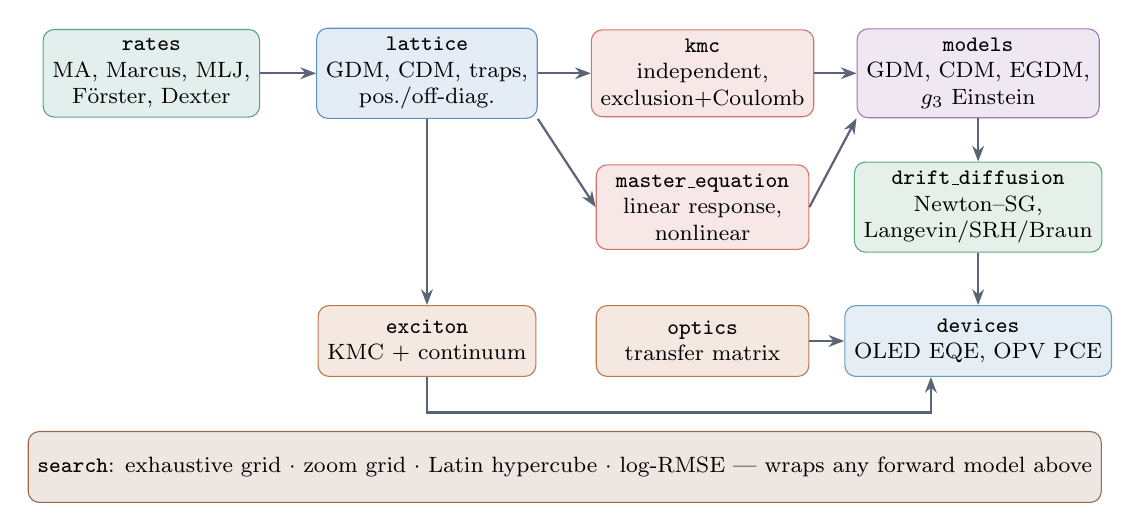
\begin{tikzpicture}[arr/.style={-{Stealth[length=2mm]},thick,draw=oDark!70}]
\node[box=cW]  (rates) at (0,0)     {\texttt{rates}\\MA, Marcus, MLJ,\\Förster, Dexter};
\node[box=cE]  (lat)   at (3.5,0)   {\texttt{lattice}\\GDM, CDM, traps,\\pos./off-diag.};
\node[box=cMu] (kmc)   at (7,0)     {\texttt{kmc}\\independent,\\exclusion+Coulomb};
\node[box=cN]  (mod)   at (10.5,0)  {\texttt{models}\\GDM, CDM, EGDM,\\$g_3$ Einstein};
\node[box=cMu] (me)    at (7,-1.7)  {\texttt{master\_equation}\\linear response,\\nonlinear};
\node[box=cF]  (dd)    at (10.5,-1.7){\texttt{drift\_diffusion}\\Newton--SG,\\Langevin/SRH/Braun};
\node[box=cG]  (exc)   at (3.5,-3.4){\texttt{exciton}\\KMC + continuum};
\node[box=cG]  (opt)   at (7,-3.4)  {\texttt{optics}\\transfer matrix};
\node[box=cJ]  (dev)   at (10.5,-3.4){\texttt{devices}\\OLED EQE, OPV PCE};
\node[box=cOp,minimum width=128mm] (search) at (5.25,-5.0) {\texttt{search}: exhaustive grid $\cdot$ zoom grid $\cdot$ Latin hypercube $\cdot$ log-RMSE --- wraps any forward model above};
\draw[arr] (rates) -- (lat);
\draw[arr] (lat) -- (kmc);
\draw[arr] (lat.south east) -- (me.west);
\draw[arr] (lat) -- (exc);
\draw[arr] (kmc) -- (mod);
\draw[arr] (me.east) -- (mod.south west);
\draw[arr] (mod) -- (dd);
\draw[arr] (dd) -- (dev);
\draw[arr] (opt) -- (dev);
\draw[arr] (exc.south) -- ++(0,-0.45) -| ([xshift=-6mm]dev.south);
\end{tikzpicture}
\end{frame}

\begin{frame}{Colour code used in every equation}
\begin{columns}
\column{0.5\textwidth}
\begin{itemize}
\item \En{energies}: $\En{E_i}$, $\En{\sigma}$, $\En{\lambda}$, $\En{E_F}$, $\En{E_g}$
\item \Mu{mobility \& diffusion}: $\Mu{\mu}$, $\Mu{D}$, $\Mu{g_3}$
\item \Fd{field \& potential}: $\Fd{F}$, $\Fd{\psi}$, $\Fd{V}$
\item \Tk{temperature}: $\Tk{T}$, $\kT$, $\Tk{V_t}$
\item \Dn{densities \& occupations}: $\Dn{n}$, $\Dn{p}$, $\Dn{f_i}$, $\Dn{N_t}$
\end{itemize}
\column{0.5\textwidth}
\begin{itemize}
\item \Rt{rates \& conductances}: $\Rt{W_{ij}}$, $\Rt{\nu_0}$, $\Rt{G_{ij}}$
\item \Js{currents}: $\Js{J_n}$, $\Js{J_p}$, $\Js{I_{ij}}$
\item \GR{generation / recombination}: $\GR{G}$, $\GR{R}$, $\GR{\gamma}$
\item \Gx{geometry}: $\Gx{r_{ij}}$, $\Gx{a}$, $\Gx{x}$, $\Gx{L}$
\item \textcolor{cOp}{operators}: $\Op{\nabla}$, $\Op{\partial}$, $\Op{\sum}$
\end{itemize}
\end{columns}
\vspace{4mm}
Reduced disorder $\sh=\En{\sigma}/\kT$. SI units throughout, energies in eV.
\end{frame}

% =====================================================================
\section{Microscopic layer: hopping rates}

\begin{frame}{Charge-transfer rates (\texttt{orchid.rates})}
\small
\textbf{Miller--Abrahams} (phonon-assisted tunnelling, weak e--ph coupling):
\[
\Rt{W_{ij}}=\Rt{\nu_0}\,e^{-2\alpha \Gx{r_{ij}}}\times
\begin{cases} e^{-\Delta\En{E_{ij}}/\kT}, & \Delta\En{E_{ij}}>0\\ 1,&\Delta\En{E_{ij}}\le0\end{cases},
\qquad \Delta\En{E_{ij}}=\En{E_j}-\En{E_i}-e\,\Fd{\mathbf F}\!\cdot\!\Gx{\mathbf r_{ij}}
\]
\textbf{Marcus} (small polaron, classical modes, reorganisation $\En{\lambda}$, transfer integral $\En{J_{ij}}$):
\[
\Rt{W_{ij}}=\frac{2\pi}{\hbar}\frac{|\En{J_{ij}}|^2}{\sqrt{4\pi\En{\lambda}\kT}}
\exp\!\left[-\frac{(\Delta\En{E_{ij}}+\En{\lambda})^2}{4\En{\lambda}\kT}\right]
\]
\textbf{Marcus--Levich--Jortner} (one quantum mode $\hbar\omega$, Huang--Rhys $S$):
\[
\Rt{W_{ij}}=\frac{2\pi}{\hbar}\frac{|\En{J_{ij}}|^2}{\sqrt{4\pi\En{\lambda_s}\kT}}\Op{\sum_{n\ge0}}
e^{-S}\frac{S^n}{n!}\exp\!\left[-\frac{(\Delta\En{E_{ij}}+\En{\lambda_s}+n\hbar\omega)^2}{4\En{\lambda_s}\kT}\right]
\]
Coupling decay for lattice use: $\En{J_{ij}}=\En{J_0}\,e^{-\alpha(\Gx{r_{ij}}-\Gx{a})}$; off-diagonal disorder multiplies $\Rt{W_{ij}}$ by $e^{\Gamma_i+\Gamma_j}$.
\end{frame}

\begin{frame}{Exciton transfer \& detailed balance}
\textbf{Förster} (dipole--dipole, singlets) and \textbf{Dexter} (exchange, triplets):
\[
\Rt{k^{F}_{ij}}=\frac{1}{\tau}\left(\frac{\Gx{R_0}}{\Gx{r_{ij}}}\right)^{6} b(\Delta\En{E}),\qquad
\Rt{k^{D}_{ij}}=\Rt{k_D}\,e^{-2\Gx{r_{ij}}/\Gx{L}}\, b(\Delta\En{E}),\qquad
b=\min\{1,e^{-\Delta\En{E}/\kT}\}
\]
\textbf{Detailed balance} (required for an equilibrium ME / Fermi--Dirac steady state):
\[
\frac{\Rt{W_{ij}}}{\Rt{W_{ji}}}=e^{-(\En{E_j}-\En{E_i})/\kT}
\]
\begin{itemize}
\item Verified to machine precision for MA, symmetric MA and Marcus in the test suite.
\item The textbook MLJ form (emission only into the quantum mode, $\hbar\omega\gg\kT$) is \alert{not} exactly detailed-balanced $\Rightarrow$ flagged in the docstring; the test checks the $S\to0$ Marcus limit instead.
\item Marcus shows the \alert{inverted region} for $\Delta\En{E}<-\En{\lambda}$ (validated: maximum at $-\En{\lambda}$ to $10^{-3}$\,eV).
\end{itemize}
\end{frame}

% =====================================================================
\section{Disordered lattices}

\begin{frame}{Energetic landscape (\texttt{orchid.lattice})}
\small
Periodic simple-cubic box $L_x\times L_y\times L_z$, lattice constant $\Gx{a}=\Dn{N_t}^{-1/3}$, neighbour table for $0<|\Gx{\mathbf r}|\le r_c$ ($r_c=\sqrt3\,\Gx a$: 26 neighbours, as Pasveer 2005).
\begin{description}
\item[GDM] $\Dn{g}(\En E)=\dfrac{\Dn{N_t}}{\sqrt{2\pi}\En{\sigma}}\exp\!\left(-\dfrac{\En{E}^2}{2\En{\sigma}^2}\right)$, uncorrelated (Bässler 1993).
\item[CDM] random permanent dipoles $\mathbf d_k$ on every site,
$\En{E_i}\propto \Op{\sum_{k\neq i}}\dfrac{\mathbf d_k\cdot(\Gx{\mathbf r_i}-\Gx{\mathbf r_k})}{|\Gx{\mathbf r_i}-\Gx{\mathbf r_k}|^3}$, computed as an FFT convolution with the minimum-image kernel, rescaled to $\En{\sigma}$ (Dunlap/Novikov).
\item[Smoothed] Gaussian-filtered white noise, correlation length $\xi$.
\item[Exponential] $\Dn{g}(\En E)\propto e^{\En{E}/\En{E_0}}$ (multiple-trapping / Vissenberg--Matters regime).
\item[Host--guest] fraction $c$ of trap/emitter sites at depth $\En{E_{tr}}$ with own width.
\item[Positional] $\Gx{\mathbf r_i}\to\Gx{\mathbf r_i}+\mathbf u_i$, $\mathbf u_i\sim\mathcal N(0,\Sigma_r^2)$.
\item[Off-diagonal] $\ln\Rt{W_{ij}}\to\ln\Rt{W_{ij}}+\Gamma_i+\Gamma_j$, $\mathrm{Var}(\Gamma)=\Sigma^2/2$.
\end{description}
Data layout: \texttt{nbr[N,M]}, \texttt{disp[N,M,3]}, \texttt{dist[N,M]} --- fully vectorised rate tables.
\end{frame}

% =====================================================================
\section{Kinetic Monte Carlo}

\begin{frame}{KMC algorithm (rejection-free, BKL / Gillespie)}
\begin{columns}[T]
\column{0.55\textwidth}\small
For a carrier on site $i$ with escape rate $\Rt{\Gamma_i}=\Op{\sum_m}\Rt{W_{i,m}}$:
\begin{enumerate}
\item waiting time $\Delta t=-\ln(1-u_1)/\Rt{\Gamma_i}$
\item choose hop $m$: smallest $m$ with $\Rt{C_{i,m}}\ge u_2\Rt{\Gamma_i}$ (\alert{binary search} in pre-computed cumulative table $\Rt{C}$)
\item update position (unwrapped $x$ for drift), time, observables
\end{enumerate}
Independent carriers: static rates $\Rightarrow$ $\mathcal O(\log M)$ per hop; carriers run in parallel (\texttt{numba.prange}, one RNG stream per carrier).\\[2mm]
Measured throughput: $\approx2\times10^{7}$ hops/s on 2 cores.
\column{0.42\textwidth}\small
\textbf{Mobility estimator} (ratio of ensemble sums, after equilibration):
\[
\Mu{\mu}=\frac{\Gx{a}\Op{\sum_c}\Delta x_c}{\Fd{F}\Op{\sum_c}\Delta t_c}
\]
Correct time average for an ergodic ensemble; avoids the bias of averaging $\Delta x_c/\Delta t_c$ when rare deep traps dominate.
\\[2mm]
\textbf{Observables on a log time grid}: $\langle x\rangle(t)$ (TOF photocurrent $I\propto d\langle x\rangle/dt$) and $\langle\En{E}\rangle(t)$ (energetic relaxation).
\end{columns}
\end{frame}

\begin{frame}{Interacting KMC: exclusion and Coulomb}
\small
Many carriers (density $\Dn{p}\Gx{a}^3$) on the same lattice:
\begin{itemize}
\item \textbf{Site exclusion}: hops to occupied sites have zero rate $\Rightarrow$ Fermi--Dirac statistics emerge, no mean-field assumption.
\item \textbf{Screened Coulomb} within cutoff $r_C$: site potential maintained incrementally,
\[
\Fd{\phi_k}\mathrel{+}=\pm\frac{e}{4\pi\varepsilon_0\varepsilon_r|\Gx{\mathbf r_k}-\Gx{\mathbf r_s}|}\quad\text{for } |\Gx{\mathbf r_k}-\Gx{\mathbf r_s}|\le r_C
\]
on every hop ($\mathcal O(r_C^3)$ instead of $\mathcal O(N)$).
\item \textbf{Self-interaction removal}: the hop energy uses
$\Delta\En{E}=\En{E_j}-\En{E_i}-e\Fd{F}\Delta x+\big[\Fd{\phi_j}-\Fd{\phi_i}-V(\Gx{r_{ij}})\big]$, the first $M$ stencil entries coincide with the hopping offsets so $V(\Gx{r_{ij}})$ is a table lookup.
\item Rates recomputed for all carriers each step: $\mathcal O(N_c M)$; adequate up to $\sim10^3$ carriers.
\end{itemize}
Result (V2): exclusion KMC reproduces the Fermi--Dirac ME within 1--7\,\% over $\Dn{p}\Gx a^3=10^{-3}\ldots10^{-1}$; switching on Coulomb lowers $\Mu\mu$ at $10^{-2}$ by $\sim2\times$ in our test, the known trend of Coulomb-enhanced disorder.
\end{frame}

% =====================================================================
\section{Master equation}

\begin{frame}{Mean-field master equation}
Steady-state occupation probabilities $\Dn{p_i}$ (Yu \emph{et al.} PRB 63, 085202; Pasveer \emph{et al.} PRL 94, 206601):
\[
\Op{\sum_j}\Big[\Rt{W_{ij}}\,\Dn{p_i}(1-\Dn{p_j})-\Rt{W_{ji}}\,\Dn{p_j}(1-\Dn{p_i})\Big]=0,\qquad \Op{\sum_i}\Dn{p_i}=\Dn{p}\,N
\]
\textbf{Nonlinear solver} (\texttt{me\_nonlinear}) --- self-consistent iteration with carrier-number renormalisation:
\[
\Dn{p_i}\leftarrow\frac{\Op{\sum_j}\Rt{W_{ji}}\Dn{p_j}}{\Op{\sum_j}\big[\Rt{W_{ij}}(1-\Dn{p_j})+\Rt{W_{ji}}\Dn{p_j}\big]},\qquad
\Dn{p_i}\leftarrow\Dn{p_i}\frac{\Dn pN}{\Op{\sum_k}\Dn{p_k}}
\]
Mobility from net bond currents $\Js{I_{ij}}$:
\[
\Mu{\mu}=\frac{\Gx a^2}{\Fd{F}\Gx a}\,\frac{\tfrac12\Op{\sum_{ij}}\Js{I_{ij}}\Delta x_{ij}}{\Op{\sum_i}\Dn{p_i}}
\]
Test: agrees with the linear-response solver to $<0.5\,\%$ at $e\Fd F\Gx a=2$\,meV.
\end{frame}

\begin{frame}{Exact linear response = Miller--Abrahams resistor network}
\small
Linearise around equilibrium $\Dn{f_i}=[1+e^{(\En{E_i}-\En{E_F})/\kT}]^{-1}$. Detailed balance makes the bond conductance symmetric:
\[
\Rt{G_{ij}}=\frac{\Rt{W^0_{ij}}\,\Dn{f_i}(1-\Dn{f_j})}{\kT}=\Rt{G_{ji}}
\]
With electrochemical potential $\En{\mu_i}=-e\Fd F x_i+\eta_i$ ($\eta$ periodic) the bond current is
$\Js{I_{ij}}=\Rt{G_{ij}}\big(\eta_i-\eta_j+e\Fd F\,\Delta x_{ij}\big)$ and Kirchhoff's law gives a sparse graph Laplacian:
\[
\Op{\sum_j}\Rt{G_{ij}}(\eta_i-\eta_j)=-e\Fd F\Op{\sum_j}\Rt{G_{ij}}\Delta x_{ij}
\]
\begin{itemize}
\item Symmetric positive semi-definite $\Rightarrow$ pin one node, \alert{Jacobi-preconditioned CG}.
\item $\En{E_F}$ from $\Op{\sum_i}\Dn{f_i}=\Dn pN$ for the actual sample (Brent).
\item Cost: $50^3$ sites, $\sh=3$: $\sim$13\,s; no time-stepping, no noise --- ideal for $\Mu\mu(\Dn p)$ tables feeding DD.
\item Sanity check: ordered lattice gives $\Mu\mu=\Mu D/(\kT/e)$ with $\Mu D=\Rt{\nu_0}e^{-2\alpha \Gx a}\Gx a^2$ to $10^{-5}$.
\end{itemize}
\end{frame}

% =====================================================================
\section{Analytical mobility models}

\begin{frame}{Parametrised mobility laws (\texttt{orchid.models})}
\small
\textbf{GDM} (Bässler 1993), $\Fd F$ in V/cm, $C=2.9\times10^{-4}$:
\[
\Mu{\mu}=\Mu{\mu_\infty}\exp\!\Big[-\big(\tfrac23\sh\big)^2\Big]\exp\!\Big[C\big(\sh^{2}-\Sigma^2\big)\sqrt{\Fd F}\Big]
\]
\textbf{CDM} (Novikov \emph{et al.} PRL 81, 4472 (1998)):
$\ \Mu{\mu}=\Mu{\mu_\infty}\exp\!\big[-(\tfrac35\sh)^2+0.78(\sh^{3/2}-2)\sqrt{e\Gx a\Fd F/\En\sigma}\big]$
\\[2mm]
\textbf{EGDM} (Pasveer \emph{et al.} 2005): $\Mu{\mu}(\Tk T,\Dn p,\Fd F)=\Mu{\mu_0}(\Tk T)\,g_1(\Dn p,\Tk T)\,g_2(\Fd F,\Tk T)$
\begin{align*}
\Mu{\mu_0}(\Tk T)&=\Mu{\mu_0}\,c_1\,e^{-c_2\sh^2},\quad c_1=1.8\times10^{-9},\ c_2=0.42,\quad \Mu{\mu_0}=\frac{\Gx a^2\Rt{\nu_0}e}{\En\sigma}\\
g_1&=\exp\!\Big[\tfrac12(\sh^2-\sh)(2\Dn p\Gx a^3)^{\delta}\Big],\quad
\delta=\frac{2}{\sh^2}\Big[\ln(\sh^2-\sh)-\ln\ln4\Big]\\
g_2&=\exp\!\Big\{0.44\big(\sh^{3/2}-2.2\big)\Big[\sqrt{1+0.8\big(e\Fd F\Gx a/\En\sigma\big)^2}-1\Big\}\Big]
\end{align*}
Also: Poole--Frenkel, Arrhenius, Vissenberg--Matters percolation conductivity for an exponential DOS.
\end{frame}

\begin{frame}{Gaussian-DOS statistics and the generalised Einstein relation}
\small
Carrier density for Fermi level $\En{E_F}$:
\[
\Dn{n}(\En{E_F})=\int \frac{\Dn{g}(\En E)\,d\En E}{1+e^{(\En E-\En{E_F})/\kT}}
\quad\Rightarrow\quad \En{E_F}(\Dn n)\ \text{by root finding (adaptive quadrature)}
\]
Diffusion enhancement in a degenerate (Gaussian) DOS:
\[
\Mu{g_3}\equiv\frac{\Mu D}{\Mu\mu\,\kT/e}=\frac{\Dn n}{\kT}\left(\frac{\partial\Dn n}{\partial\En{E_F}}\right)^{-1}
\]
\begin{itemize}
\item $\Mu{g_3}\to1$ in the Boltzmann limit (tested to 1\,\%); $\Mu{g_3}>1.5$ at $\Dn n\Gx a^3=10^{-2}$, $\sh=3.9$.
\item Single-carrier equilibrium energy $\langle\En E\rangle_\infty=-\En\sigma^2/\kT$ (used in V4).
\item Tabulated $\Mu{g_3}(\Dn n)$ is passed directly to the DD solver.
\end{itemize}
\end{frame}

% =====================================================================
\section{Drift--diffusion device solver}

\begin{frame}{Governing equations}
\[
\Op{\nabla}\cdot(\varepsilon\Op{\nabla}\Fd\psi)=-e\big(\Dn p-\Dn n+N_D^+-N_A^-\big)-\rho_t
\]
\[
\Op{\partial_x}\Js{J_n}=e(\GR R-\GR G),\qquad \Op{\partial_x}\Js{J_p}=-e(\GR R-\GR G)
\]
\[
\Js{J_n}=e\Mu{\mu_n}\Dn n\Fd F+e\Mu{D_n}\Op{\partial_x}\Dn n,\qquad
\Js{J_p}=e\Mu{\mu_p}\Dn p\Fd F-e\Mu{D_p}\Op{\partial_x}\Dn p,\qquad \Mu{D}=\Mu{g_3}\Mu\mu\Tk{V_t}
\]
\begin{itemize}
\item $\Mu\mu$ may be constant, Poole--Frenkel, EGDM $\Mu\mu(\Dn p,\Fd F,\Tk T)$ or any user callable --- evaluated on edges with mean density and edge field.
\item $\rho_t$: trapped charge from SRH single-level occupation (acceptor/donor-like).
\item Contacts: Dirichlet $\Dn n,\Dn p$ from injection barriers (Boltzmann), $\Fd\psi(L)-\Fd\psi(0)=V_{bi}-\Fd V$, $V_{bi}=\En{E_g}-\varphi_p^{A}-\varphi_n^{C}$.
\end{itemize}
\end{frame}

\begin{frame}{Discretisation: Scharfetter--Gummel with generalised Einstein}
\small
On edge $i+\tfrac12$ of length $h_i$, $\Delta=(\Fd{\psi_{i+1}}-\Fd{\psi_i})/\Tk{V_t}$, Bernoulli $B(x)=x/(e^x-1)$:
\[
\Js{J_{n,i+\frac12}}=\frac{e\Mu{\mu_n}\Mu{g_3}\Tk{V_t}}{h_i}\Big[\Dn{n_{i+1}}B\!\big(\tfrac{\Delta}{\Mu{g_3}}\big)-\Dn{n_i}B\!\big(-\tfrac{\Delta}{\Mu{g_3}}\big)\Big],\quad
\Js{J_{p,i+\frac12}}=\frac{e\Mu{\mu_p}\Mu{g_3}\Tk{V_t}}{h_i}\Big[\Dn{p_i}B\!\big(\tfrac{\Delta}{\Mu{g_3}}\big)-\Dn{p_{i+1}}B\!\big(-\tfrac{\Delta}{\Mu{g_3}}\big)\Big]
\]
\begin{itemize}
\item Exact for constant current \& field on each edge; upwinds automatically at high field, central at low field.
\item Overflow-safe $B(x)=x e^{-x}/(1-e^{-x})$ for $x>0$, Taylor series for $|x|<10^{-6}$.
\item \textbf{Non-uniform tanh grid} refined at both contacts: $x=\tfrac L2\big[1+\tanh(\beta(2s-1))/\tanh\beta\big]$; box-integration with dual cells $\tfrac12(h_{i-1}+h_i)$. Essential: uniform grids fail to resolve the minority-carrier boundary layer above $V_{bi}$.
\end{itemize}
\end{frame}

\begin{frame}{Fully coupled Newton solver}
\small
\begin{itemize}
\item Unknowns per node: $\Fd\psi$, $u=\ln(\Dn n/N_c)$, $v=\ln(\Dn p/N_v)$ $\Rightarrow$ positivity by construction; densities may span $>40$ decades.
\item Continuity rows scaled by the local density (same root, far better conditioning).
\item Interleaved ordering $[\psi_1,u_1,v_1,\psi_2,\dots]$: each residual depends on nodes $i-1,i,i+1$ $\Rightarrow$ \alert{banded Jacobian, bandwidth 5}.
\item Jacobian by \alert{11-colour finite differences}: perturb every 11th unknown simultaneously $\Rightarrow$ only 11 residual evaluations per Jacobian, \emph{independent of grid size} and of the mobility law (EGDM, user callables work unchanged).
\item Banded LU (\texttt{scipy.linalg.solve\_banded}); damping limits $|\delta\psi|/\Tk{V_t},|\delta u|,|\delta v|\le2$.
\item Voltage continuation from equilibrium in both directions, adaptive step (\(\times1.5\) on success, \(/3\) on failure).
\end{itemize}
Performance: 31-point $J$--$V$ on 201 nodes in $\approx1$\,s; current continuity $\mathrm{std}(\Js J)/\langle\Js J\rangle<10^{-6}$.
\end{frame}

\begin{frame}{Recombination, generation and dissociation}
\small
\textbf{Langevin} (reduction factor $\zeta$): $\GR{R_L}=\zeta\,\dfrac{e(\Mu{\mu_n}+\Mu{\mu_p})}{\varepsilon}\big(\Dn n\Dn p-\Dn{n_i}^2\big)$
\\[1mm]
\textbf{SRH / trap-assisted} with trapped charge:
\[
\GR{R_{SRH}}=\frac{C_nC_p\Dn{N_t}(\Dn n\Dn p-\Dn{n_i}^2)}{C_n(\Dn n+\Dn{n_1})+C_p(\Dn p+\Dn{p_1})},\qquad
\Dn{f_t}=\frac{C_n\Dn n+C_p\Dn{p_1}}{C_n(\Dn n+\Dn{n_1})+C_p(\Dn p+\Dn{p_1})}
\]
\textbf{Braun--Onsager CT dissociation} (Koster \emph{et al.} PRB 72, 085205 (2005) scheme): $\GR{G}\to P\GR G$, $\GR R\to(1-P)\GR R$
\[
P=\frac{\Rt{k_d}}{\Rt{k_d}+\Rt{k_f}},\quad
\Rt{k_d}=\frac{3\GR\gamma}{4\pi \Gx{a_{CT}}^3}e^{-\En{E_b}/\kT}\frac{J_1(2\sqrt{-2b})}{\sqrt{-2b}},\quad
b=\frac{e^3\Fd F}{8\pi\varepsilon(\kT)^2},\quad \En{E_b}=\frac{e^2}{4\pi\varepsilon \Gx{a_{CT}}}
\]
\textbf{Generation}: uniform, Beer--Lambert, or transfer-matrix profile $\GR{G}(x)$.
\end{frame}

% =====================================================================
\section{Optics, excitons and device workflows}

\begin{frame}{Transfer-matrix optics (\texttt{orchid.optics})}
\small
Pettersson, Roman \& Inganäs, J.\ Appl.\ Phys.\ 86, 487 (1999); complex index $\tilde n_j=n_j+ik_j$:
\[
\mathbf I_{jk}=\frac1{t_{jk}}\begin{pmatrix}1&r_{jk}\\ r_{jk}&1\end{pmatrix},\quad
\mathbf L_j=\begin{pmatrix}e^{-i\xi_jd_j}&0\\0&e^{i\xi_jd_j}\end{pmatrix},\quad \xi_j=\frac{2\pi\tilde n_j}{\lambda}
\]
Field inside layer $j$ ($\mathbf S',\mathbf S''$: partial products left/right):
\[
E_j(\Gx x)=t_j^{+}\big[e^{i\xi_j\Gx x}+r''_j e^{i\xi_j(2d_j-\Gx x)}\big],\quad t_j^+=\big[S'_{11}+S'_{12}r''_je^{2i\xi_jd_j}\big]^{-1}
\]
\[
Q_j(\Gx x,\lambda)=\tfrac12c\varepsilon_0\,\alpha_jn_j|E_j|^2,\quad \alpha_j=\frac{4\pi k_j}{\lambda},\qquad
\GR{G}(\Gx x)=\int Q_j(\Gx x,\lambda)\frac{\lambda}{hc}\,d\lambda
\]
Lorentz-oscillator absorber model; placeholder 5778\,K spectrum scaled to 1000\,W\,m$^{-2}$ (load ASTM G173 for quantitative work). OLED escape cone: $\eta_{out}\approx1/(2n^2)$.
\end{frame}

\begin{frame}{Excitons: KMC and continuum (\texttt{orchid.exciton})}
\small
\textbf{KMC}: exciton walks with Förster/Dexter rates until decay ($k_d=1/\tau$, competing channel in the BKL step).
\[
\langle\Gx r^2\rangle=6\Mu D\tau,\qquad L_D=\sqrt{\Mu D\tau},\qquad \Mu{D}_{\sigma=0}=\tfrac16\Op{\sum_j}\Rt{k_j}\Gx{r_j}^2\ \text{(exact check)}
\]
\textbf{Continuum emission zone} (Newton on the DD grid):
\[
0=\Mu D\,\Op{\partial_x^2}S+\eta\,\GR{R}(\Gx x)-\frac S\tau-k_{SS}S^2-k_{SP}(\Dn n+\Dn p)S,\qquad S=0\ \text{at metal (quenching)}
\]
\textbf{OLED EQE}:
\[
\mathrm{EQE}=\underbrace{\frac{e\int\GR R\,d\Gx x}{\Js J}}_{\gamma_b}\ \eta_{S/T}\ \underbrace{q_{PL}\frac{\int S/\tau\,d\Gx x}{\int\GR R\,d\Gx x}}_{q_{\rm eff}}\ \eta_{out}
\]
Captures charge balance, emission-zone position, electrode quenching and annihilation-driven roll-off.
\end{frame}

% =====================================================================
\section{Exhaustive search}

\begin{frame}{Exhaustive search engine (\texttt{orchid.search})}
\small
\begin{itemize}
\item \textbf{Full grid}: Cartesian product of candidate values; every point stored $\Rightarrow$ the complete objective \emph{landscape} (identifiability, degeneracies, multiple minima are visible --- unlike local optimisers).
\item \textbf{Zoom grid}: repeat the full grid in a box shrunk ($\times0.35$) around the incumbent; log-space axes for scale parameters ($\Mu{\mu}$, $\Rt{\nu_0}$, $\Dn{N_t}$).
\item \textbf{Latin hypercube}: space-filling screening of high-dimensional design spaces.
\item \textbf{Objective}: log-RMSE, $\sqrt{\langle(\log_{10}y_{model}-\log_{10}y_{data})^2\rangle}$ --- natural for $\Mu\mu$ and $\Js J$ spanning decades.
\item Embarrassingly parallel (\texttt{ProcessPoolExecutor}); any ORCHID solver (KMC, ME, DD, optics) can be the forward model.
\end{itemize}
Use cases: GDM/EGDM parameters from $\Mu\mu(\Tk T,\Fd F)$ or temperature-dependent SCLC; $\Mu{\mu_p}$ and injection barrier from $J$--$V$; screening layer thickness, offsets and mobilities for maximum PCE or balanced OLED transport.
\end{frame}

% =====================================================================
\section{Validation against published results}

\begin{frame}{Validation matrix}
\scriptsize\setlength{\tabcolsep}{4pt}
\begin{tabular}{@{}llll@{}}
\toprule
\# & Quantity & Reference & Outcome\\
\midrule
V1 & $\Mu\mu(\Tk T)$, $\Dn p\to0$ & EGDM, Pasveer PRL 94, 206601 (2005) & ME$=$KMC (3--10\,\%); $\le1.2\times$ EGDM for $\sh\le3$\\
V2 & $\Mu\mu(\Dn p)$ & EGDM $g_1$ & ME$=$exclusion KMC (1--7\,\%); EGDM for $\sh=3,4$\\
V3 & $\Mu\mu(\Fd F)$ & EGDM $g_2$ & quantitative at $\sh=3$; $\pm30$\,\% at $\sh=2,4$\\
V4 & $\langle\En E\rangle_\infty$ & $-\En\sigma^2/\kT$ (Bässler 1993) & 1.7\,\% at $\sh=2$; finite-sample limit at $\sh=3$\\
V5 & SCLC & Mott--Gurney & $\Js J/\Js J_{MG}\to1.06$ at 40\,V\\
V6 & $V_{oc}(\GR G)$ & Koster APL 86, 123509 (2005) & $\le1.3$\,mV, slope $1.004\,\kT/e$\\
V7 & exciton $\Mu D$ & $\tfrac16\sum k r^2$ (exact) & within statistical error\\
V8 & optics & Airy formula; $R+T+A=1$ & $10^{-16}$; $10^{-5}$\\
V9 & inverse problems & synthetic ground truth & $\En\sigma$, $\Mu{\mu_\infty}$, $\Sigma$ within 1\,\%\\
V10 & TOF transients & dispersive transport (Scher--Montroll) & plateau tilts, tail broadens with $\sh$\\
V11 & Marcus vs MA & inverted region, detailed balance & $7\times10^{-15}$\\
V12 & OLED / OPV & device physics trends & roll-off, emission zone, PCE\\
\bottomrule
\end{tabular}
\end{frame}

\begin{frame}{V1 --- temperature dependence vs Pasveer \emph{et al.} (2005)}
\begin{columns}[c]
\column{0.55\textwidth}
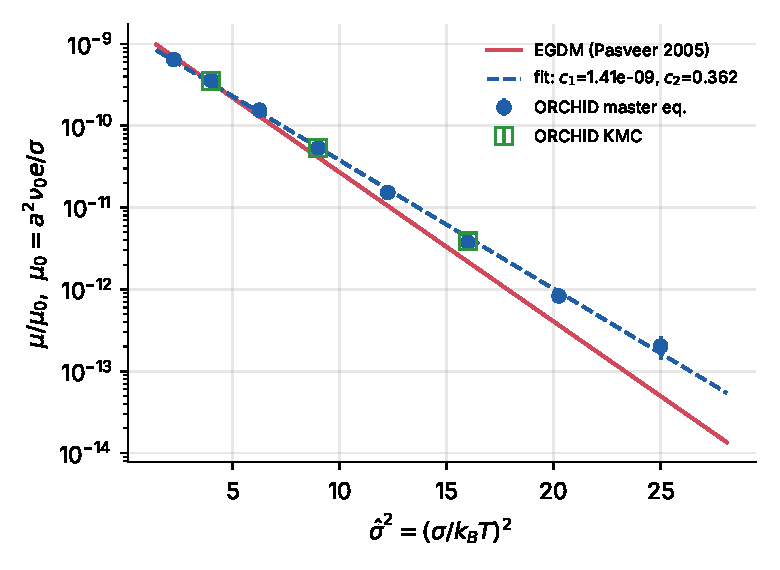
\includegraphics[width=\linewidth]{v1_mobility_temperature.pdf}
\column{0.43\textwidth}\small
\begin{itemize}
\item Same model as Pasveer: cubic lattice, $\alpha\Gx a=10$, $r_c=\sqrt3\Gx a$, MA rates.
\item ME ($50^3$, 3 samples) and KMC ($30^3$) agree within 3--10\,\% $\Rightarrow$ the two independent solvers cross-validate.
\item Exhaustive grid fit over $\sh\in[1.5,5]$: $c_1=1.41\times10^{-9}$ (paper: $1.8\times10^{-9}$), $c_2=0.36$ (paper: 0.42; Bässler: $4/9$).
\item Deviation grows with $\sh$: at $\sh\ge4$ the box cannot hold enough sites near $-\En\sigma^2/\kT$ (need $N\gg e^{\sh^2/2}$) $\Rightarrow$ finite samples overestimate $\Mu\mu$. Pasveer extrapolated in size; we report raw results honestly.
\end{itemize}
\end{columns}
\end{frame}

\begin{frame}{V2 --- carrier-density dependence (EGDM $g_1$)}
\begin{columns}[c]
\column{0.55\textwidth}
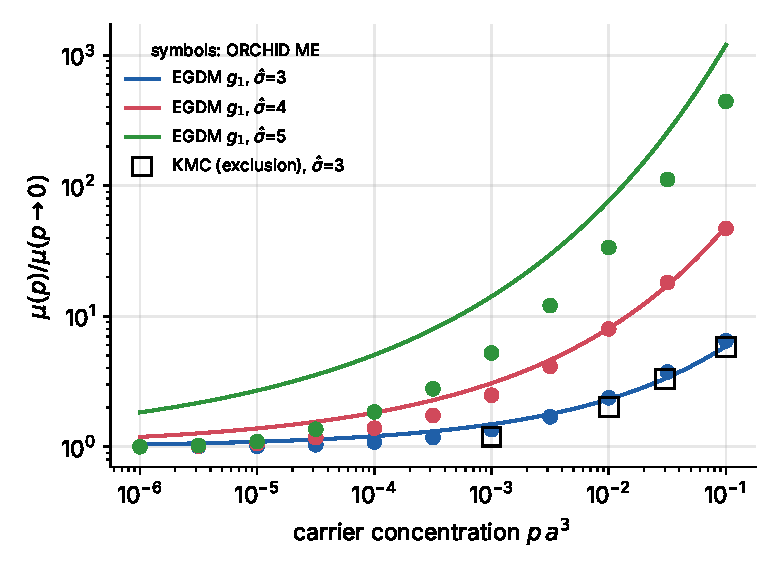
\includegraphics[width=\linewidth]{v2_density.pdf}
\column{0.43\textwidth}\small
\begin{itemize}
\item Fermi--Dirac ME ($40^3$, 2 samples) reproduces $g_1$ quantitatively for $\sh=3$ and 4 over five decades of $\Dn p$.
\item Many-particle KMC with site exclusion ($24^3$, up to 1382 carriers) matches the mean-field ME within 1--7\,\% $\Rightarrow$ the mean-field approximation is accurate here.
\item $\sh=5$: shape is right but normalisation by the (finite-size-inflated) $\Dn p\to0$ value compresses the curve --- same origin as V1.
\end{itemize}
\end{columns}
\end{frame}

\begin{frame}{V3 --- field dependence (EGDM $g_2$)}
\begin{columns}[c]
\column{0.55\textwidth}
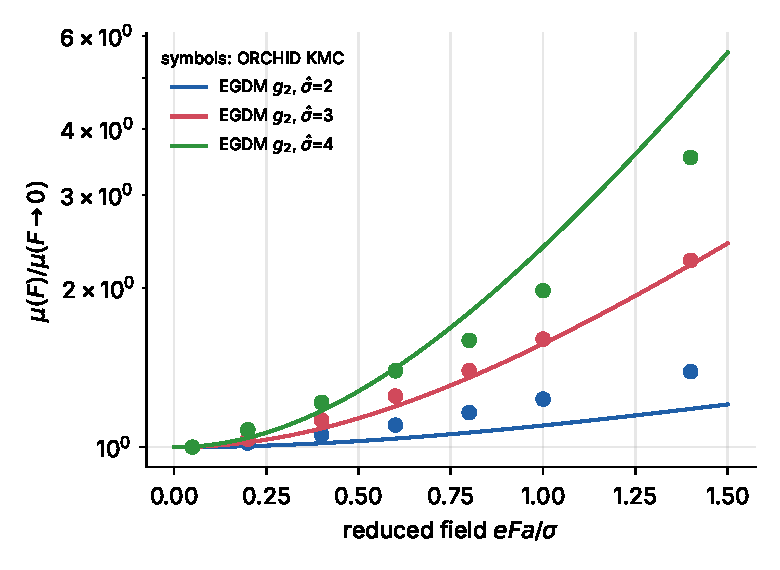
\includegraphics[width=\linewidth]{v3_field.pdf}
\column{0.43\textwidth}\small
\begin{itemize}
\item Independent-carrier KMC on $30^3$ sites, $e\Fd F\Gx a/\En\sigma=0.05$--1.4.
\item Quantitative at $\sh=3$; KMC is stronger than $g_2$ at $\sh=2$ and weaker at $\sh=4$ (within $\sim30$\,\%).
\item Expected: $g_2$ was fitted at finite density and in a limited $\sh$ window; the prefactor $(\sh^{3/2}-2.2)$ nearly vanishes at $\sh=2$.
\item Field heating and finite-size effects are both captured directly by KMC.
\end{itemize}
\end{columns}
\end{frame}

\begin{frame}{V4 \& V10 --- relaxation and time of flight}
\begin{columns}[c]
\column{0.5\textwidth}
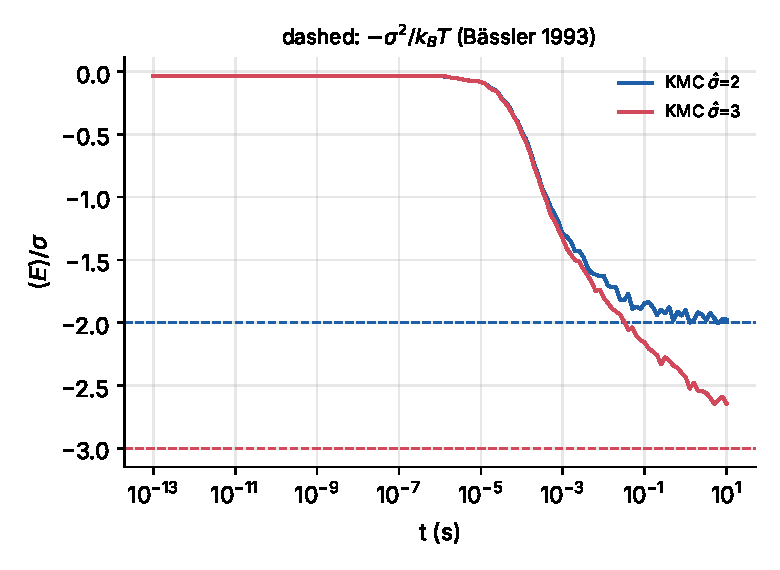
\includegraphics[width=0.8\linewidth]{v4_relaxation.pdf}
\column{0.5\textwidth}
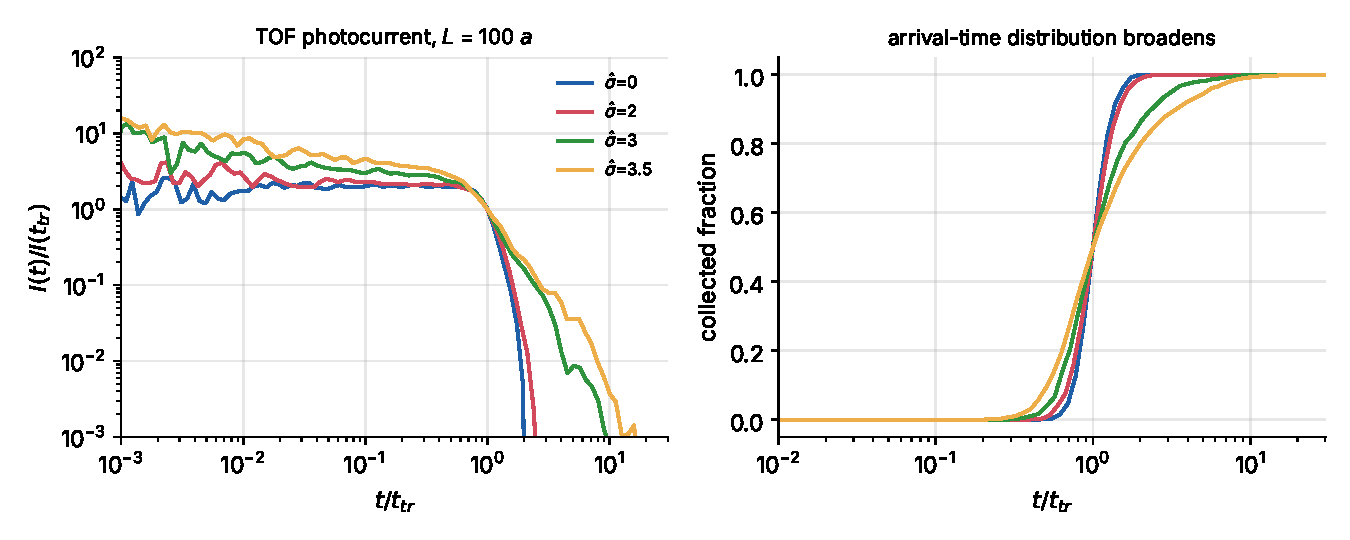
\includegraphics[width=\linewidth]{v10_tof.pdf}
\end{columns}
\small
Left: mean energy relaxes to $-\En\sigma^2/\kT$ (dashed). At $\sh=2$: $-1.97\En\sigma$ vs $-2\En\sigma$. At $\sh=3$ the $40^3$ sample's own Boltzmann mean is $-2.73\En\sigma$ (finite-size limit); KMC reaches $-2.57\En\sigma$ inside the time window.
Right: TOF ($L=100\,\Gx a$, $e\Fd F\Gx a=0.4\kT$) in universal scaling: a flat plateau with a sharp cut-off at $\sh=0$; with growing $\sh$ the plateau tilts and the arrival tail broadens --- the onset of dispersive transport.
\end{frame}

\begin{frame}{V5 --- space-charge-limited current}
\centering
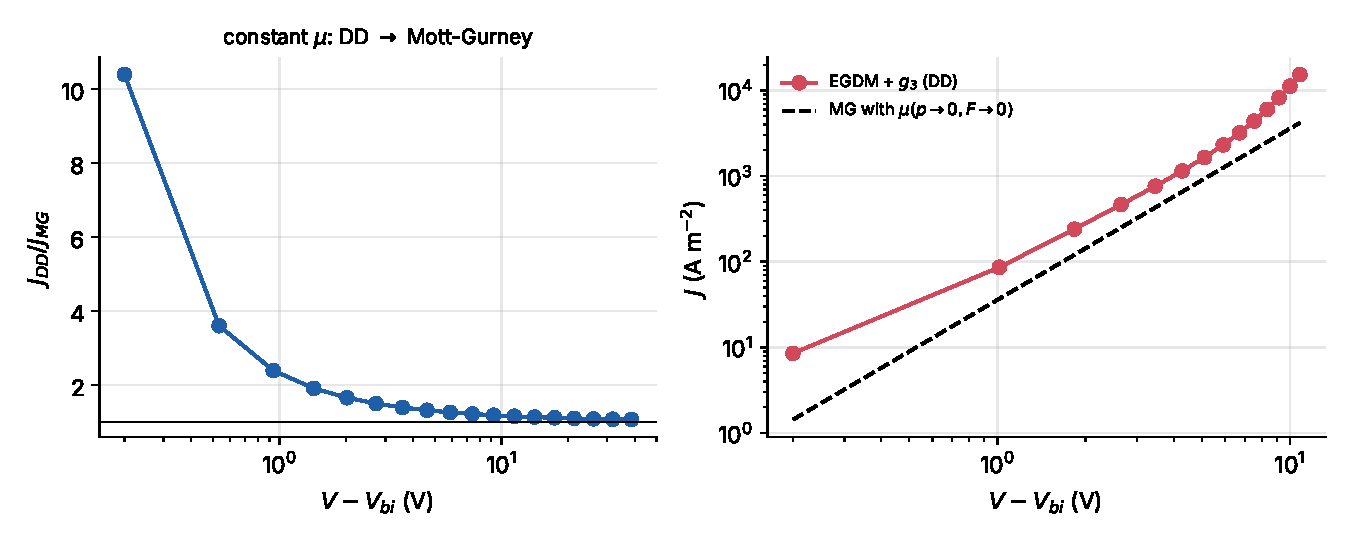
\includegraphics[width=0.8\linewidth]{v5_sclc.pdf}\\
\footnotesize
Left: hole-only diode (Ohmic anode, 1.4\,eV blocking cathode). DD approaches Mott--Gurney $\Js J=\tfrac98\varepsilon\Mu\mu(\Fd V-V_{bi})^2/\Gx L^3$ from above (diffusion correction), 1.06 at 40\,V.
Right: EGDM + $\Mu{g_3}$: the density and field dependence lift $\Js J$ well above the constant-$\Mu\mu$ MG law and raise the slope (cf.\ van Mensfoort \& Coehoorn, PRB 78, 085207 (2008)).
\end{frame}

\begin{frame}{V6 --- open-circuit voltage vs Koster \emph{et al.} (2005)}
\begin{columns}[c]
\column{0.55\textwidth}
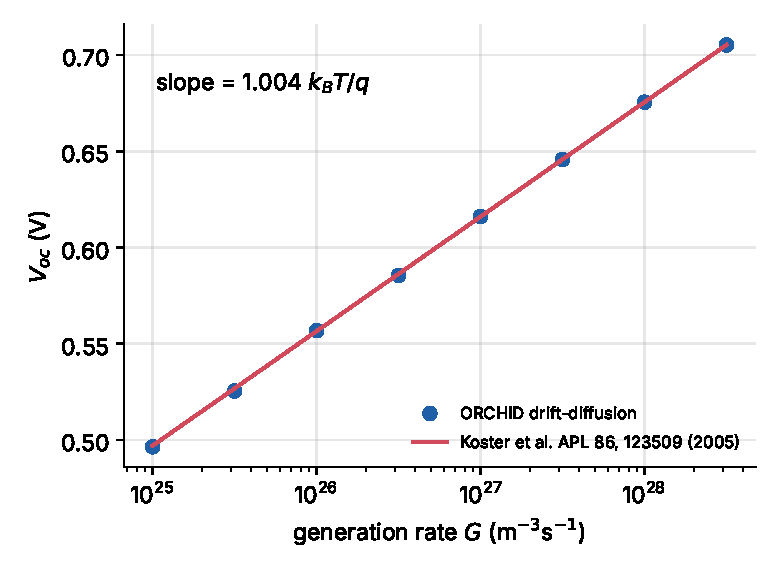
\includegraphics[width=\linewidth]{v6_voc.pdf}
\column{0.43\textwidth}\footnotesize
Analytical result for Langevin recombination of free carriers:
\[
V_{oc}=\frac{\En{E_g}}{e}-\frac{\kT}{e}\ln\frac{\GR{\gamma}N_c^2}{\GR G}
\]
\begin{itemize}
\item ORCHID DD reproduces it within $\le1.3$\,mV over 3.5 decades of $\GR G$ ($V_{oc}$ from a monotone-cubic interpolant of $J(V)$).
\item Light-intensity slope $=1.004\,\kT/e$ per $e$-fold: the bimolecular-recombination signature (Koster \emph{et al.}).
\item Validates Poisson/continuity coupling, recombination and contact treatment together.
\end{itemize}
\end{columns}
\end{frame}

\begin{frame}{V7 \& V8 --- excitons and optics}
\begin{columns}[c]
\column{0.5\textwidth}
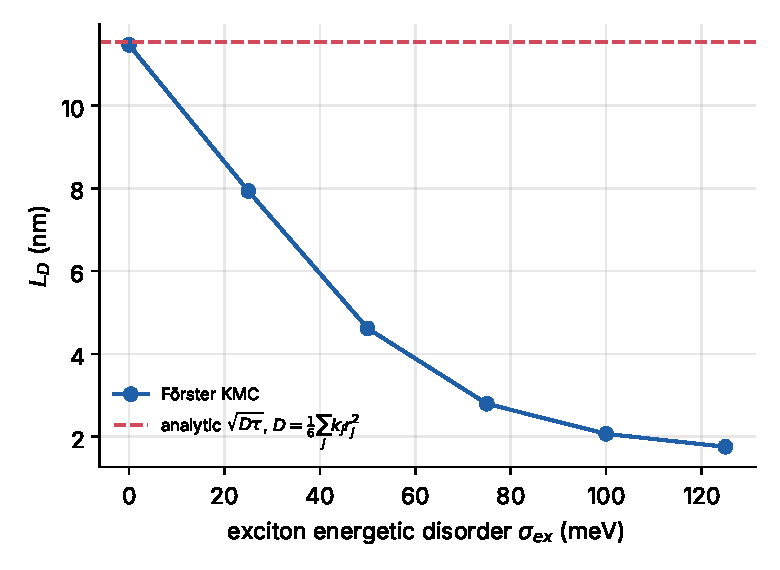
\includegraphics[width=\linewidth]{v7_exciton.pdf}
\column{0.5\textwidth}
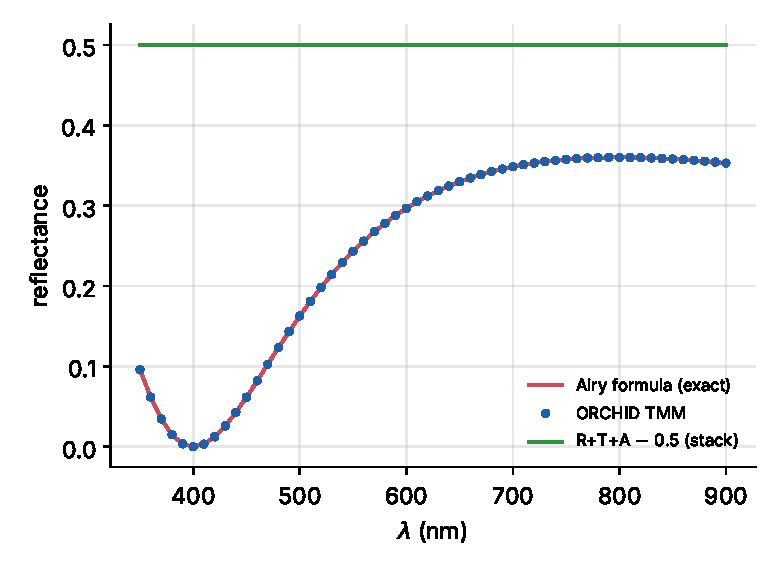
\includegraphics[width=\linewidth]{v8_tmm.pdf}
\end{columns}
\small
Left: Förster KMC ($R_0=2$\,nm, $\tau=1$\,ns) gives the exact $\Mu D=\tfrac16\sum\Rt{k_j}\Gx{r_j}^2$ without disorder; $L_D$ falls as $\En{\sigma_{ex}}$ grows (downhill trapping).
Right: TMM agrees with the Airy formula to machine precision; energy is conserved in an ITO/PEDOT/blend/Al stack.
\end{frame}

\begin{frame}{V9 --- exhaustive-search inversion}
\centering
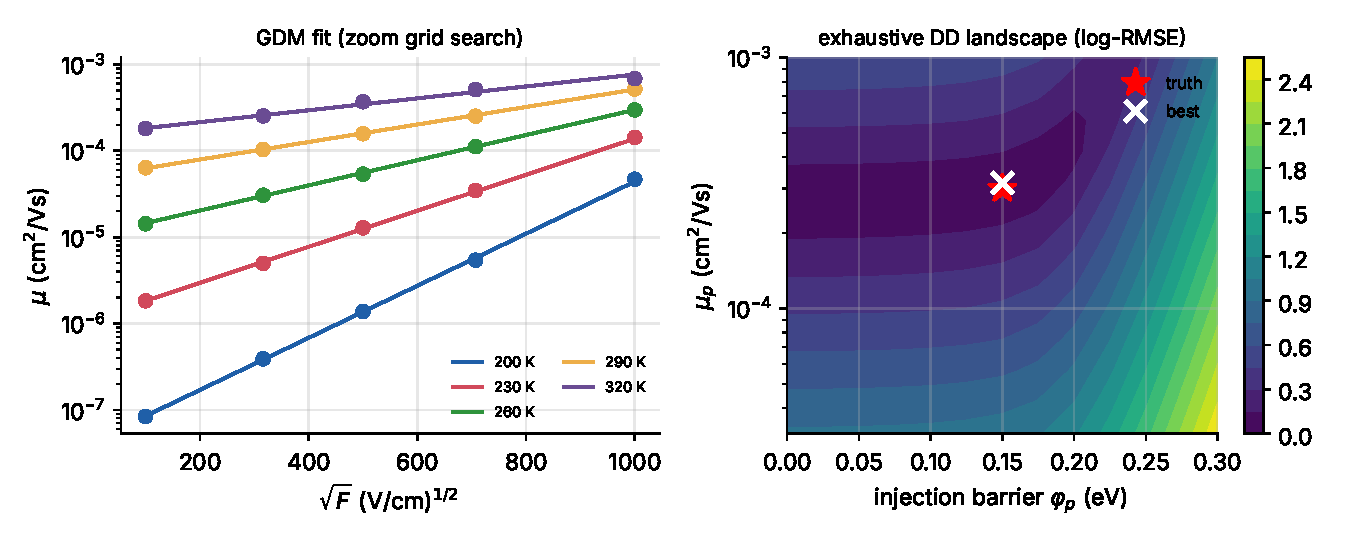
\includegraphics[width=0.8\linewidth]{v9_search.pdf}\\
\footnotesize
Left: GDM recovered from synthetic $\Mu\mu(\Tk T,\Fd F)$ with 5\,\% noise by a 5-level zoom grid ($15^3$ points/level): $\En\sigma=94.9$ (true 95)\,meV, $\Mu{\mu_\infty}=0.0302$ (0.030)\,cm$^2$/Vs, $\Sigma=2.52$ (2.5).
Right: full $13\times13$ DD landscape for $(\varphi_p,\Mu{\mu_p})$ from a noisy hole-only $J$--$V$; the minimum lands on the true barrier (0.15\,eV) and the grid point nearest the true mobility. The valley shape shows the barrier/mobility correlation, which a local optimiser would hide.
\end{frame}

\begin{frame}{V11 --- Marcus vs Miller--Abrahams}
\centering
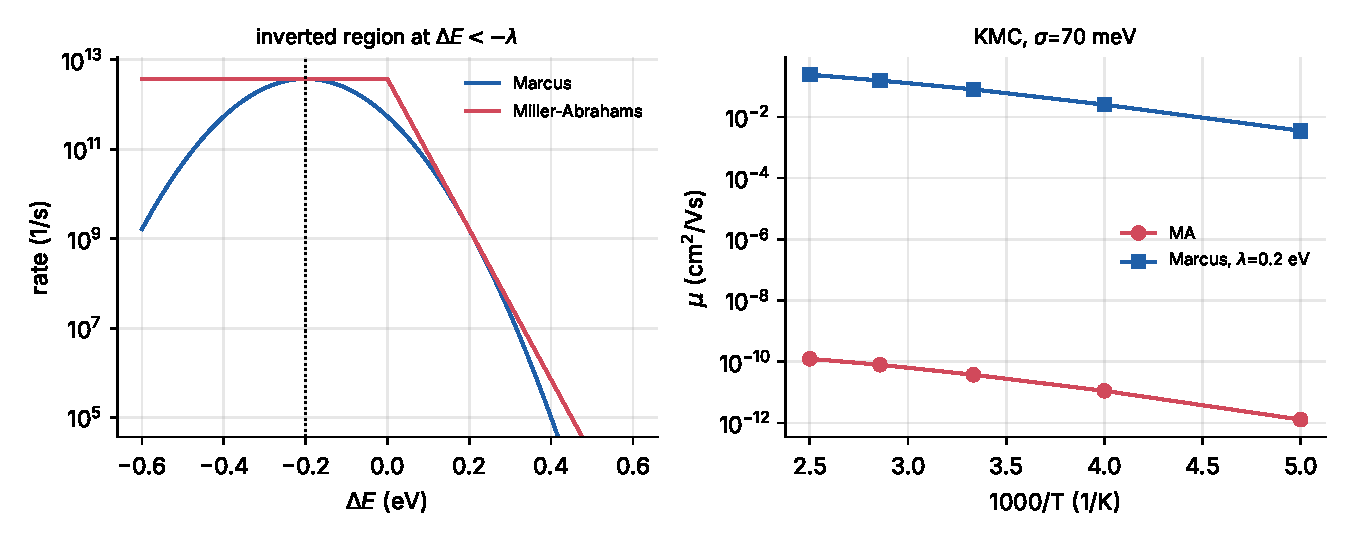
\includegraphics[width=0.8\linewidth]{v11_marcus.pdf}\\
\footnotesize
Left: rates vs $\Delta\En E$ --- Marcus has an inverted region below $-\En\lambda$, while MA saturates.
Right: KMC on the same $\En\sigma=70$\,meV landscape. Effective activation 0.159\,eV (MA) vs 0.146\,eV (Marcus, $\En\lambda=0.2$\,eV). The polaron term $\sim\En\lambda/4$ is offset by a weaker disorder penalty, because Marcus downhill rates are not saturated (cf.\ Fishchuk \emph{et al.} 2003). Absolute prefactors use different conventions ($\Rt{\nu_0}e^{-2\alpha a}$ vs $\En{J_0}$), so compare slopes only.
\end{frame}

\begin{frame}{V12a --- organic solar cell with transfer-matrix optics}
\centering
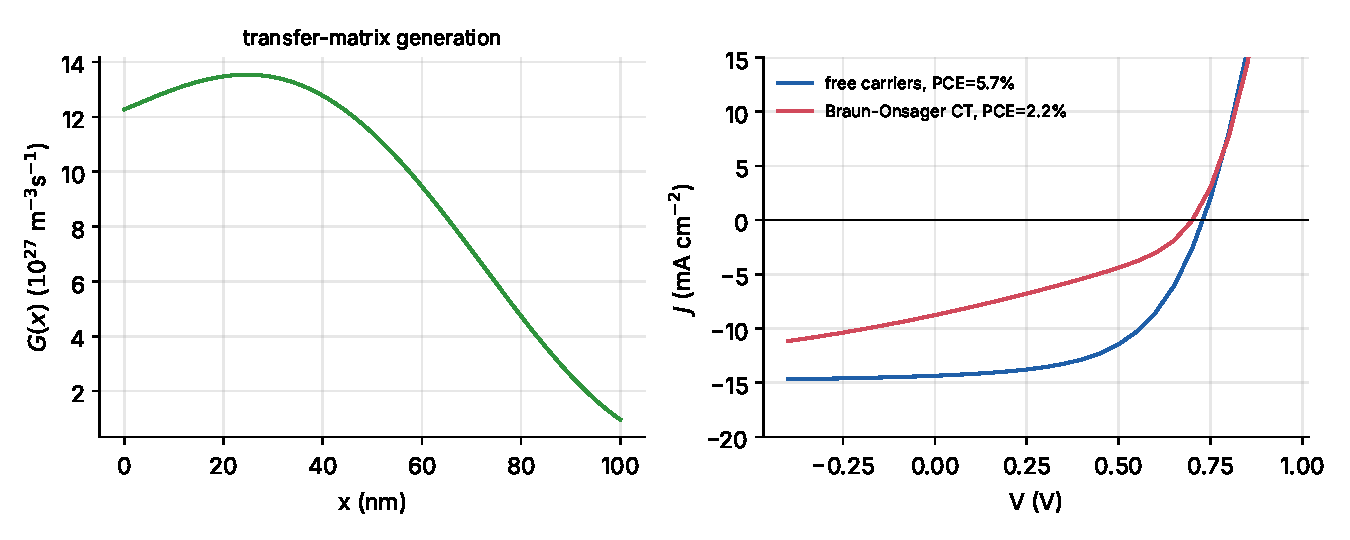
\includegraphics[width=0.8\linewidth]{v12_opv.pdf}\\
\footnotesize
Stack glass/ITO(120)/PEDOT:PSS(40)/blend(100, Lorentz absorber)/Al(100\,nm). Left: TMM interference profile $\GR G(\Gx x)$, with a node at the Al mirror. Right: $J$--$V$ with $\zeta=0.1$ reduced Langevin. Free-carrier generation: $J_{sc}=14.4$\,mA\,cm$^{-2}$, $V_{oc}=0.73$\,V, FF\,$=0.55$, PCE\,$=5.7$\,\%. Braun--Onsager CT dissociation ($a_{CT}=1.5$\,nm, $k_f=10^6$\,s$^{-1}$) adds field-dependent geminate loss: $J_{sc}=8.8$\,mA\,cm$^{-2}$, FF\,$=0.36$, PCE\,$=2.2$\,\%.
\end{frame}

\begin{frame}{V12b --- OLED: emission zone and efficiency roll-off}
\centering
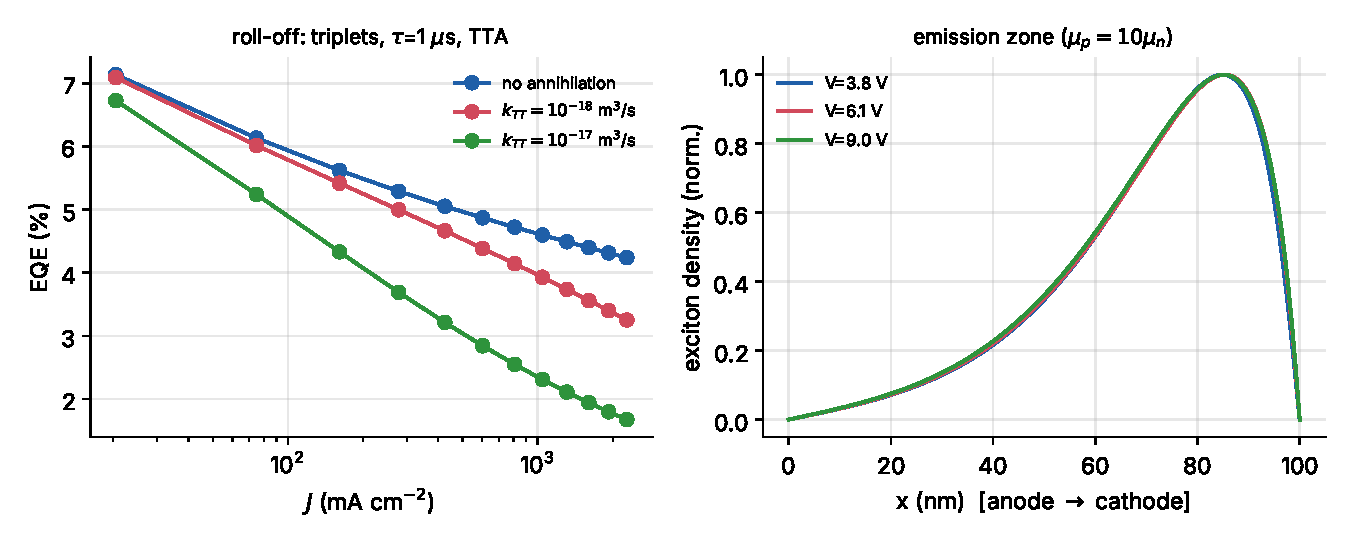
\includegraphics[width=0.8\linewidth]{v12_oled.pdf}\\
\footnotesize
Single-layer phosphorescent OLED, 100\,nm, $\Mu{\mu_p}=10\Mu{\mu_n}$, 0.1\,eV injection barriers, triplet $\tau=1\,\mu$s, $L_D=20$\,nm, $\eta_{S/T}=1$, $q_{PL}=0.9$, $\eta_{out}=1/(2n^2)$.
Left: triplet--triplet annihilation ($k_{TT}=10^{-18}$, $10^{-17}$\,m$^3$/s) drives the roll-off; without TTA the residual decline comes from charge-balance loss and electrode quenching.
Right: the recombination zone sits about 15\,nm from the cathode (slow electrons) and barely moves with bias.
\end{frame}

% =====================================================================
\section{Software engineering}

\begin{frame}[fragile]{Repository layout \& quality}
\begin{columns}[T]
\column{0.45\textwidth}\scriptsize
\begin{verbatim}
orchid/
  orchid/   rates.py  lattice.py
            kmc.py    master_equation.py
            models.py drift_diffusion.py
            exciton.py optics.py
            devices.py search.py cli.py
  tests/test_orchid.py      (22 tests)
  validation/bench_*.py     (V1-V12)
  validation/figures, results/*.json
  examples/01-04_*.py
  docs/slides/orchid_slides.tex
  .github/workflows/tests.yml
  pyproject.toml README.md LICENSE
\end{verbatim}
\column{0.52\textwidth}\small
\begin{itemize}
\item Tests: detailed balance, inverted region, lattice topology, disorder statistics, ME$\leftrightarrow$KMC, ME nonlinear$\leftrightarrow$linear, Einstein limit, Gaussian statistics, Bernoulli, Koster $V_{oc}$, current continuity, MG limit, Braun limits, TMM, excitons, search.
\item CI on Python 3.10--3.12 (GitHub Actions).
\item Numba optional at import (pure-Python fallback).
\item Every benchmark writes figures and machine-readable JSON (reproducible).
\end{itemize}
\end{columns}
\end{frame}

\begin{frame}[fragile]{Usage}
\scriptsize
\begin{verbatim}
from orchid.lattice import Lattice
from orchid.master_equation import me_linear_response
from orchid.drift_diffusion import Device
from orchid.devices import simulate_opv
from orchid.optics import lorentz_nk

lat = Lattice(40, a=1.6e-9, seed=1).set_disorder(0.1, model="dipolar")
mu, info = me_linear_response(lat, T=300, n_frac=1e-3, alpha=10.0)

dev = Device(L=100e-9, Eg=1.2, mu_n=1e-8, mu_p=1e-8, langevin_prefactor=0.1,
             braun=dict(a_ct=1.5e-9, kf=1e6))
stack = [("ITO", 1.9+0.01j, 120e-9), ("PEDOT", 1.5+0.02j, 40e-9),
         ("blend", lorentz_nk, 100e-9), ("Al", 0.96+6.69j, 100e-9)]
res = simulate_opv(dev, V=np.linspace(-0.4, 0.95, 28), layers=stack, active_index=2)
\end{verbatim}
\small Command line:
\scriptsize
\begin{verbatim}
orchid mobility --method kmc --sigma 0.1 --T 250 --density 1e-2 --coulomb
orchid jv --Eg 1.2 --G 1e27 --Vmin -0.3 --Vmax 0.9
orchid egdm --T 300 --p 1e23 --F 1e7
\end{verbatim}
\end{frame}

\section{Limitations, roadmap and next steps}

\begin{frame}{Honest limitations of v0.1}
\small
\begin{itemize}
\item \textbf{Finite-size effects} at $\sh\gtrsim4$ (V1/V2). Planned: automatic size extrapolation and larger sparse solves (AMG preconditioner).
\item \textbf{Device level is 1D} drift--diffusion; no 3D device KMC with explicit injection, image charges and multilayer morphology yet.
\item Coulomb in KMC uses a real-space cutoff (no Ewald sum); ME is mean field (no correlations), though V2 shows they are small here.
\item MLJ in the low-temperature form; no Gaussian-DOS (Paasch--Scheinert) contact statistics in DD; Boltzmann contacts only.
\item Optics: coherent layers only, placeholder solar spectrum, no dipole-emission microcavity model for OLED outcoupling.
\item No transient DD (TPC/TPV, impedance), no OFET 2D geometry, no ab initio morphology / transfer-integral pipeline yet.
\end{itemize}
These are explicit targets, not hidden assumptions.
\end{frame}

\begin{frame}{Roadmap toward a complete reference platform}
\small
\begin{enumerate}
\item 3D device KMC (injection, extraction, exciton formation, TTA/TPQ, multilayer OLED stacks)
\item Ewald / image-charge Coulomb; correlated disorder from real dipole fields; ECDM parametrisation
\item Transient \& small-signal DD (TPC, TPV, CELIV, impedance spectroscopy); 2D DD for OFETs and bulk heterojunction morphologies
\item Dipole-emitter optics (Chance--Prock--Silbey) for OLED outcoupling; ASTM G173 spectrum and $n,k$ database
\item Morphology input (MD snapshots) + DFT transfer integrals / site energies (VOTCA-like) $\to$ parameter-free mobilities
\item ML surrogates of $\Mu\mu(\Tk T,\Dn p,\Fd F)$ trained on ORCHID ME/KMC data; Bayesian inversion on top of exhaustive grids
\item GPU kernels (CuPy) for KMC and ME
\end{enumerate}
\end{frame}

\begin{frame}{Tomorrow: publishing to GitHub}
\small
\begin{enumerate}
\item Repository prepared locally with one initial commit on \texttt{main}.
\item Create an empty repo \texttt{Gokaran-Shukla/orchid} (public, no README).
\item \texttt{git remote add origin git@github.com:Gokaran-Shukla/orchid.git}
\item \texttt{git push -u origin main} $\Rightarrow$ CI runs the 22 tests automatically.
\item Add topics (organic-electronics, oled, kinetic-monte-carlo, drift-diffusion), a release tag \texttt{v0.1.0}, Zenodo DOI for citation.
\end{enumerate}
\end{frame}

\begin{frame}[allowframebreaks]{References}
\footnotesize
\begin{itemize}
\item H.\ Bässler, phys.\ stat.\ sol.\ (b) 175, 15 (1993) --- Gaussian disorder model.
\item A.\ Miller, E.\ Abrahams, Phys.\ Rev.\ 120, 745 (1960).
\item R.\ A.\ Marcus, Rev.\ Mod.\ Phys.\ 65, 599 (1993); J.\ Jortner, J.\ Chem.\ Phys.\ 64, 4860 (1976).
\item W.\ F.\ Pasveer \emph{et al.}, Phys.\ Rev.\ Lett.\ 94, 206601 (2005) --- EGDM.
\item R.\ Coehoorn \emph{et al.}, Phys.\ Rev.\ B 72, 155206 (2005) --- density dependence.
\item S.\ V.\ Novikov \emph{et al.}, Phys.\ Rev.\ Lett.\ 81, 4472 (1998) --- CDM.
\item M.\ Bouhassoune \emph{et al.}, Org.\ Electron.\ 10, 437 (2009) --- ECDM.
\item Z.\ G.\ Yu \emph{et al.}, Phys.\ Rev.\ B 63, 085202 (2001) --- master equation.
\item M.\ C.\ J.\ M.\ Vissenberg, M.\ Matters, Phys.\ Rev.\ B 57, 12964 (1998).
\item S.\ L.\ M.\ van Mensfoort, R.\ Coehoorn, Phys.\ Rev.\ B 78, 085207 (2008) --- EGDM in DD.
\item D.\ L.\ Scharfetter, H.\ K.\ Gummel, IEEE Trans.\ Electron Devices 16, 64 (1969).
\item L.\ J.\ A.\ Koster \emph{et al.}, Phys.\ Rev.\ B 72, 085205 (2005); Appl.\ Phys.\ Lett.\ 86, 123509 (2005).
\item C.\ L.\ Braun, J.\ Chem.\ Phys.\ 80, 4157 (1984).
\item L.\ A.\ A.\ Pettersson, L.\ S.\ Roman, O.\ Inganäs, J.\ Appl.\ Phys.\ 86, 487 (1999).
\item A.\ B.\ Bortz, M.\ H.\ Kalos, J.\ L.\ Lebowitz, J.\ Comput.\ Phys.\ 17, 10 (1975); D.\ T.\ Gillespie, J.\ Comput.\ Phys.\ 22, 403 (1976).
\item K.\ Zojer, Adv.\ Opt.\ Mater.\ 9, 2100219 (2021) --- review of KMC/ME/DD device modelling.
\item G.\ Cotelli \emph{et al.}, Phys.\ Rev.\ B 112, 035307 (2025) --- 3D KMC of rough OLED interfaces.
\item Identifying pitfalls when using the Miller--Abrahams rate in KMC, J.\ Mater.\ Chem.\ C 13, 14962 (2025).
\item H.\ Scher, E.\ W.\ Montroll, Phys.\ Rev.\ B 12, 2455 (1975) --- dispersive transport.
\item I.\ I.\ Fishchuk \emph{et al.}, Phys.\ Rev.\ B 67, 224303 (2003) --- polaron + disorder.
\end{itemize}
\end{frame}

\end{document}
